
\section{Theorie}
\label{sec:Theorie}

\subsection{Brechung und Dispersion}

Ändert eine Lichtwelle am Grenzübergang zwischen zwei Medien ihre Richtung, wird dies als Brechung bezeichnet. Die Lichtwelle ändert ihre Richtung, da sie mit den Elektronen in der Materie in Wechselwirkung tritt und dadurch ihre Ausbreitungsgeschwindigkeit geändert wird. Die Brechung wird über den Brechungsindex $n$ beschrieben, welcher definiert ist als:
\begin{equation}
n := \frac{v_1}{v_2}\text{.} \label{eq:ndef}
\end{equation}
$v_1$ und $v_2$ sind dabei die Geschwindigkeiten vor und nach der Brechung. 
Trifft die Lichtwelle also unter einem Winkel $\alpha$ auf die Grenzfläche, breitet sie sich darauf unter einem Winkel $\beta$ aus. Die Winkel werden dabei zum Lot der Grenzfläche gemessen.\\
Mithilfe des Huygensschen Prinzips, welches besagt, dass jeder Punkt einer Welle als Ursprung einer Elementarwelle gesehen werden kann, deren Einhüllende die neue Wellenfront ergibt, kann mit \eqref{eq:ndef} folgende Beziehung zwischen dem Brechungsindex und den Winkeln hergeleitet werden:
\begin{equation}
\frac{\sin\alpha}{\sin\beta} = \frac{v_1}{v_2} = n\text{.} \label{eq:Snellius}
\end{equation}
Dieser Zusammenhang wird als Snelliussches Brechungsgesetz bezeichnet.\\
Unter genauerer Betrachtung stellt sich heraus, dass der Brechungsindex von der Wellenlänge des Lichts abhängt. Dies wird als Dispersion bezeichnet und der Brechungsindex kann demnach geschrieben werden als:
\[n = n(\lambda)\text{.}\] 
$n(\lambda)$ wird Dispersionskurve genannt.

\subsection{Die Dispersionsgleichung}

Der Zusammenhang zwischen dem Brechungsindex und der Wellenlänge wird durch die Dispersionsgleichung beschrieben. Um diese herzuleiten, werden die elektrisch geladenen Bestandteile der Materie betrachtet, welche durch die elektromagnetische Lichtwelle zu erzwungenen Schwingungen angeregt werden. Dieses Modell ist nicht für Wellenlängen unterhalb des sichtbaren Spektrums gültig, da hier Quantenmechanische Effekte auftreten. Zudem muss die Wellenlänge hinreichend weit entfernt von der Resonanzwellenlänge betrachtet werden, welche aufgrund der erzwungenen Schwingungen auftritt, da hier ein Großteil des Lichtes absorbiert wird. Diese Bedingungen sind für Gläser im sichtbaren Spektralbereich erfüllt.\\
Unter Betrachtung der schwingenden Teilchen als elektrischen Dipol bestimmt sich der Brechungsindex nach längerer Rechnung unter Berücksichtigung der Maxwellschen Relation $\epsilon=n^2$ und den obigen Annahmen zu:
\begin{equation}
n^2(\lambda)=1+\sum_h\frac{N_hq^2_h}{4\pi^2 c^2\epsilon_0 m_h}\frac{\lambda^2\lambda^2_h}{\lambda^2-\lambda^2_h}\text{.}\label{eq:n^2}
\end{equation}
Dabei beschreiben $N_h$ die Anzahl pro Volumeneinheit, $q_h$ die Ladung, $m_h$ die Masse und $\lambda_h$ die Resonanzwellenlänge der Teilchenart $h$. \\
Wird Gleichung \eqref{eq:n^2} mit nur einer Resonanzfrequenz $\lambda_1$ betrachtet, so lässt sie sich für $\lambda >>\lambda_1$ schreiben als:
\begin{align}
n^2(\lambda)&=1+\frac{N_1 q_1^2 \lambda_1^2}{4\pi^2 c^2 \epsilon_0 m_1}\left(1+\left(\frac{\lambda_1}{\lambda}\right)^2+\left(\frac{\lambda_1}{\lambda}\right)^4+\ldots\right)\nonumber\\
			&=A_0+\frac{A_2}{\lambda^2}+\frac{A_4}{\lambda^4}+\ldots\label{eq:n^2 für l>>l1}
\end{align} 
und für $\lambda <<\lambda_1$ als:
\begin{align}
n^2(\lambda)&=1-\frac{N_1 q_1^2 }{4\pi^2 c^2 \epsilon_0 m_1}\left(\lambda^2+\frac{\lambda^4}{\lambda_1^2}+\frac{\lambda^6}{\lambda_1^4}+\ldots\right)\nonumber\\
			&=1-A_2^\prime\lambda^2-A_4^\prime\lambda^4-\ldots\label{eq:n^2 für l<<l1}
\end{align} 
Da bei beiden Gleichungen der Brechungsindex mit zunehmender Wellenlänge abnimmt, liegt normale Dispersion vor. Der umgekehrte Fall, wenn der Brechungsindex mit zunehmender Wellenlänge zunimmt, heißt anormale Dispersion. Sie tritt in der Nähe der Absorptionsstellen $\lambda_i$ für $\lambda <<\lambda_i$ auf.

\subsection{Brechung am Prisma}

Verläuft ein Lichtstrahl durch ein Glasprisma, so wird er zwei mal gebrochen, solange er nicht senkrecht auf das Prisma trifft (vergleiche Abbildung \ref{fig:Prisma}). Wird der symmetrische Strahlengang betrachtet, das heißt $\alpha =\alpha^\prime$ und $\beta =\beta^\prime$, ergeben sich für $\alpha$ und $\beta$:
\begin{align*}
\alpha 	&= \frac{\eta+\phi}{2}\text{,}\\
\beta 	&= \frac{\phi}{2}\text{.}
\end{align*}
Mit dem Snelliusschen Brechungsgesetz \eqref{eq:Snellius} ergibt sich somit für den Brechungsindex:
\begin{equation}
n = \frac{\sin\frac{\eta +\phi}{2}}{\sin\frac{\phi}{2}}\label{eq:n}
\end{equation}

\begin{figure}
\centering
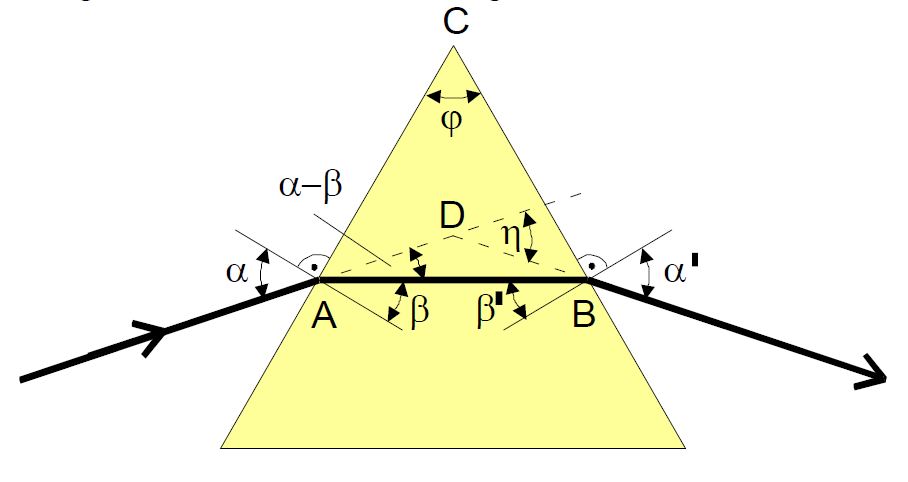
\includegraphics[width=\linewidth-70pt,height=\textheight-70pt,keepaspectratio]{content/images/Prisma.png}
\caption{Skizze des symmetrischen Strahlenganges durch das Glasprisma \cite{V402}.}
\label{fig:Prisma}
\end{figure}

\subsection{Das Auflösungsvermögen eines Prismenspektralapparates}

Unter der Auflösung $A$ eines Prismenspektralapparates versteht man das Verhältnis von der gemittelten Wellenlänge $\lambda$ zweier Spektrallinien zu dem minimalen Wellenlängenunterschied $\Delta\lambda$ dieser, sodass sie noch vom Gerät getrennt werden können:
\[
A := \frac{\lambda}{\Delta\lambda}\text{.}
\]
Das Auflösungsvermögen eines idealen Prismenspektralapparates ist durch Beugungserscheinungen am Prisma festgelegt, die aufgrund dessen endlicher Größe auftreten. Werden zwei verschiedene Wellenlängen $\lambda$ und $\lambda +\Delta\lambda$ mit dem Prismenspektralapparat vermessen, so werden diese wie in Abbildung \ref{fig:Aufloesungsvermoegen} zu sehen wegen der Wellenlängenabhängigkeit des Brechungsindexes \eqref{eq:n^2} unterschiedlich gebrochen, sodass zwei Beugungsfiguren entstehen.\\
Bei kleinem Wellenlängenunterschied $\Delta\lambda$ sind die Hauptmaxima nur leicht gegeneinander verschoben. Es soll genau dann noch eine Trennung der Linien von dem Gerät möglich sein, wenn das Maximum der einen Linie mit dem ersten Minimum der anderen übereinstimmt. Nach einiger Rechnung ergibt sich bei symmetrischem Strahlengang unter Ausnutzung von Formel \eqref{eq:n} für das Auflösungsvermögen:
\begin{equation}
A = b\frac{.dn}{.d\lambda}
\end{equation}   
Dabei stellt $b$ die Basisbreite des Prismas dar (vergleiche Abbildung \ref{fig:Aufloesungsvermoegen}). 

\begin{figure}
\centering
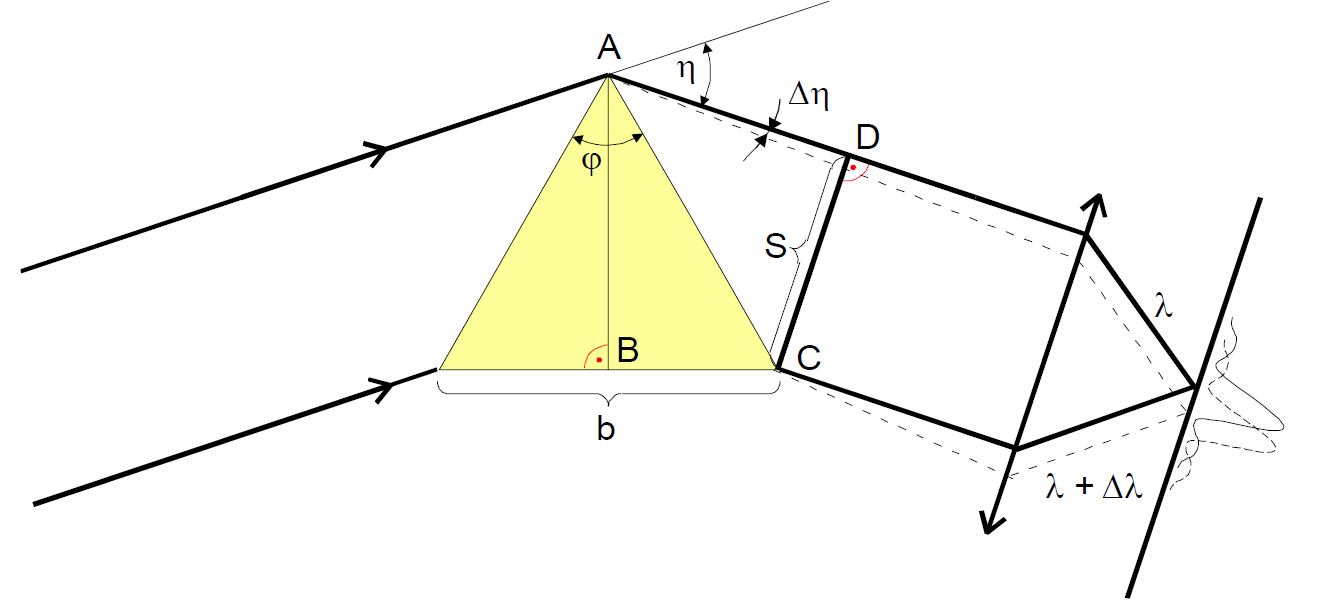
\includegraphics[width=\linewidth-50pt,height=\textheight-50pt,keepaspectratio]{content/images/Aufloesungsvermoegen.png}
\caption{Skizze für die Brechung zweier Wellenlängen $\lambda$ und $\lambda +\Delta\lambda$ beim idealen Prismenspektralapparat \cite{V402}.}
\label{fig:Aufloesungsvermoegen}
\end{figure}



